
\section{Team PML 30 ${\varphi}$} 
	Team "PML 30 ${\varphi}$" was assembled in September 2014 in  the Russian city, St. Petersburg, from 3 novices and one experienced like as captain. Among the participants were assigned tasks and roles, set safety rules. In the first place in the team was put noble professional, spread it to the masses. All decisions taken collectively in team with discussion and finding optimal solutions. 
	During the year team took part in many events and everywhere we have tried attract our team and encourage people to take a part in FTC. Also everywhere pursuing and distribution the principles of noble professional. Talking with a press, we would like attract more attention to our team and to the competition in general, as well as attracting sponsors. The last was important because of needing funds for the purchase of materials and equipment, that cost really a lot.
	Team took part in the three qualifying competitions and the regional finals. In all of them make new contacts, share experience and provide mutual assistance with other teams. In the first qualifying rounds in Sochi we have contacts "Stuy  fission 310", team from USA, and maintain contact with them untill this day. On regional finals, we met a team from Romania "Autovortex" keep in touch by Facebook. Also, there is an active dialogue with many Russian teams. Team page in Facebook you can find the desired address: https://www.facebook.com/pages/FTC-team-PML30-PHI.
	To increase the efficiency of team work, was involved version control system GitHub, which allows the entire team to work simultaneously at the same project, without losing files and easy way to resolve problems. Also for writing technical books professional typesetting system latex has been used.
	\begin{figure}[H]
		\center{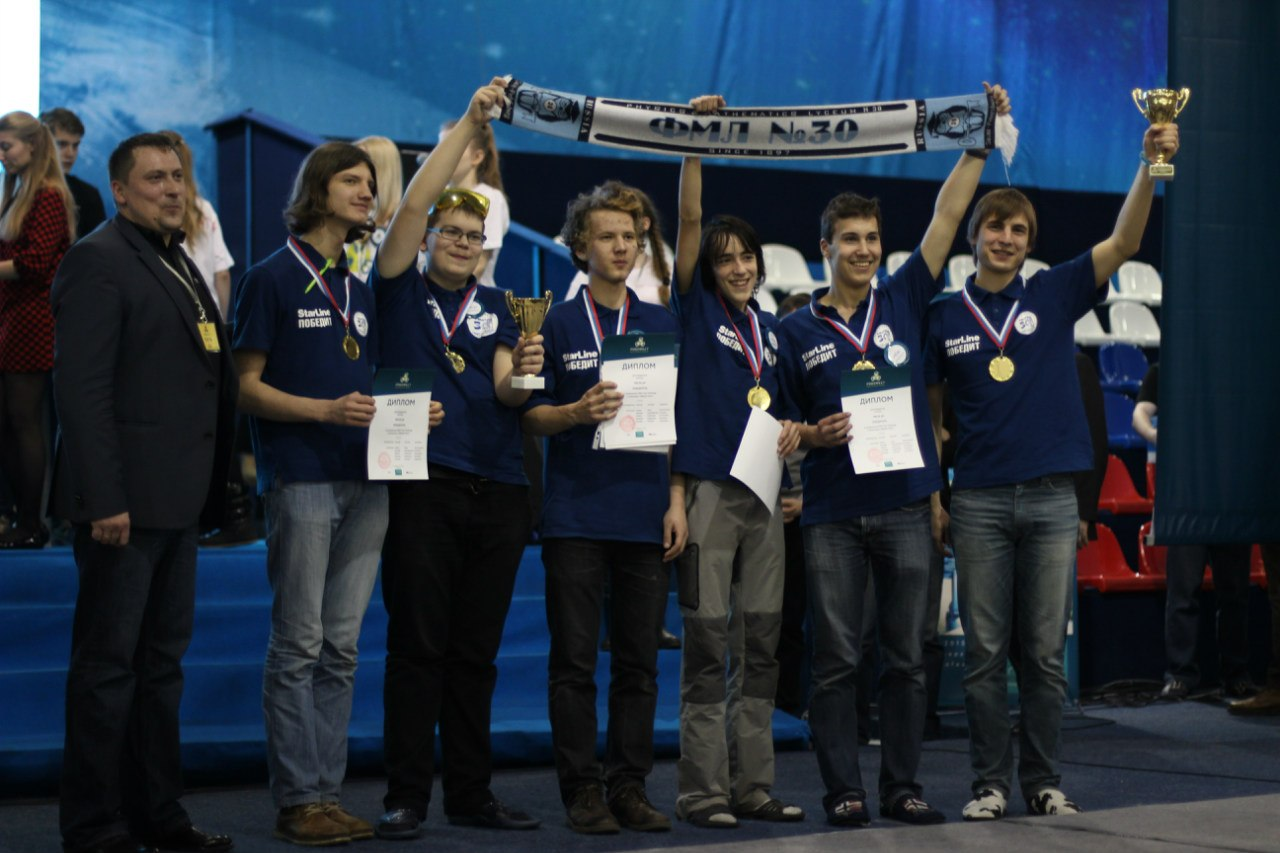
\includegraphics[scale=0.2]{days/Team/images/09}}\\
	\end{figure}[H]
\fillpage

\subsubsection{Instructors}:

\begin{figure}[H]
	
	\begin{minipage}[h]{0.47\linewidth}
		Luzin Dmitry\\
		\emph{Head of Robotics Department in Phys-Math Lyceum 30, Saint-Peterburg, Russia. Main coach of FTC team.\\}
		\emph{Information: 25 years old, in robotics 5 years, in FTC 3 years.}
	\end{minipage}
	\hfill
	\begin{minipage}{0.47\linewidth}
		\center{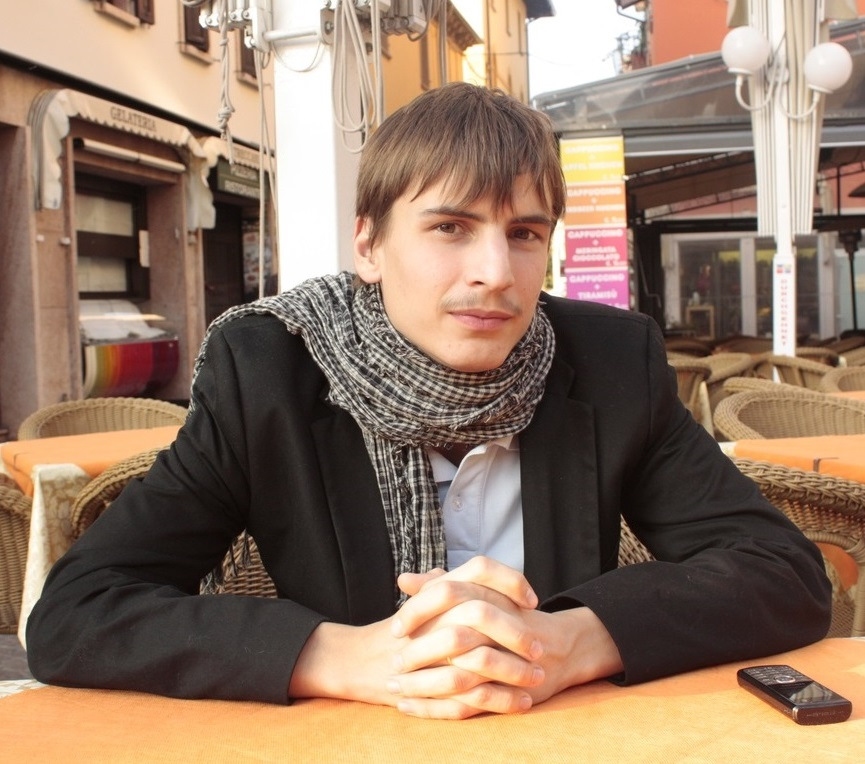
\includegraphics[scale=0.3]{days/Team/images/07}}\\
	\end{minipage}
	\vfill
	\begin{minipage}[h]{0.47\linewidth}
		\center{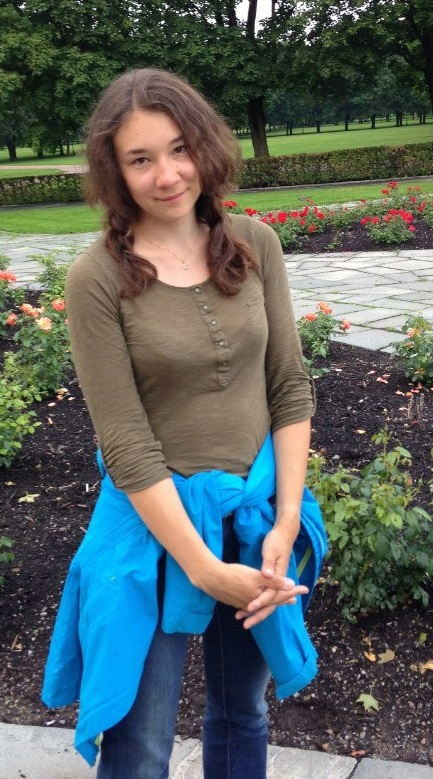
\includegraphics[scale=0.35]{days/Team/images/08}}\\
	\end{minipage}
	\hfill
	\begin{minipage}{0.47\linewidth}
		Luzina Ekaterina \\
		\emph{Professor of Robotics Department in Phys-Math Lyceum 30, Saint-Peterburg, Russia. Tutor of FTC team. \\}
		\emph{Information: 25 years old, in robotics 5 years, in FTC 3 years.}
	\end{minipage}
\end{figure}

\begin{figure}[H]
	\begin{minipage}[h]{0.47\linewidth}
		\center{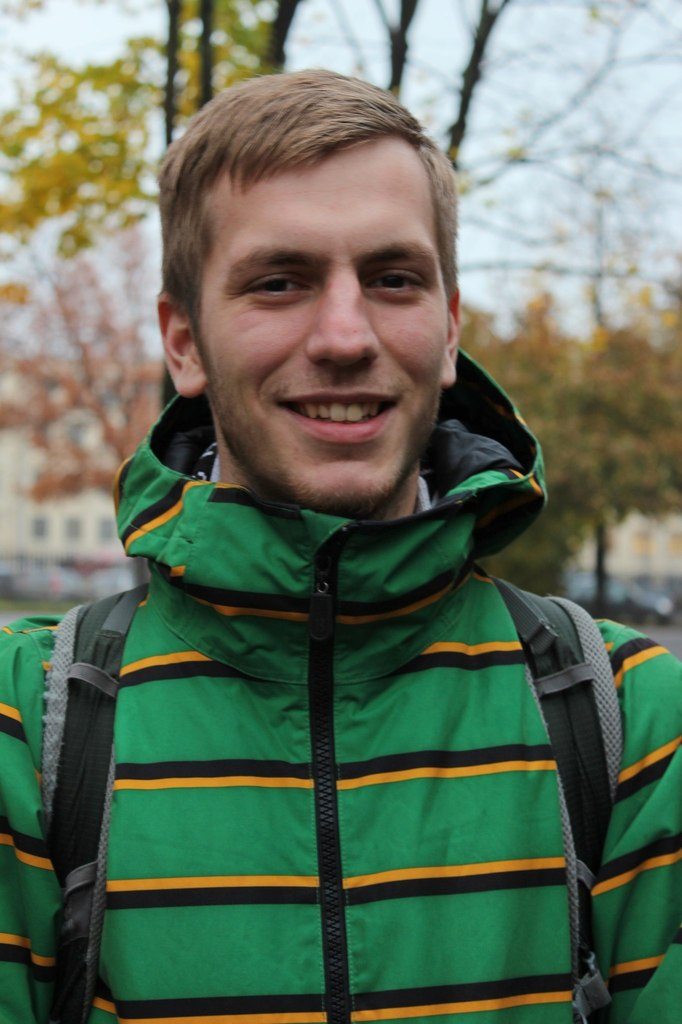
\includegraphics[scale=0.25]{days/Team/images/05}}\\
	\end{minipage}
	\hfill
	\begin{minipage}{0.47\linewidth}
		Fedotov Anton \\ 
		\emph{Professor of Robotics Department in Phys-Math Lyceum 30, Saint-Peterburg, Russia. Tutor of FTC team. \\}
		\emph{Information: 22 years old, in robotics 4 years, in FTC 3 years.}
	\end{minipage}	
	\vfill 
\end{figure}

\fillpage

\subsubsection{Team members}
\begin{figure}[H]
	\begin{minipage}[h]{0.47\linewidth}
		\center{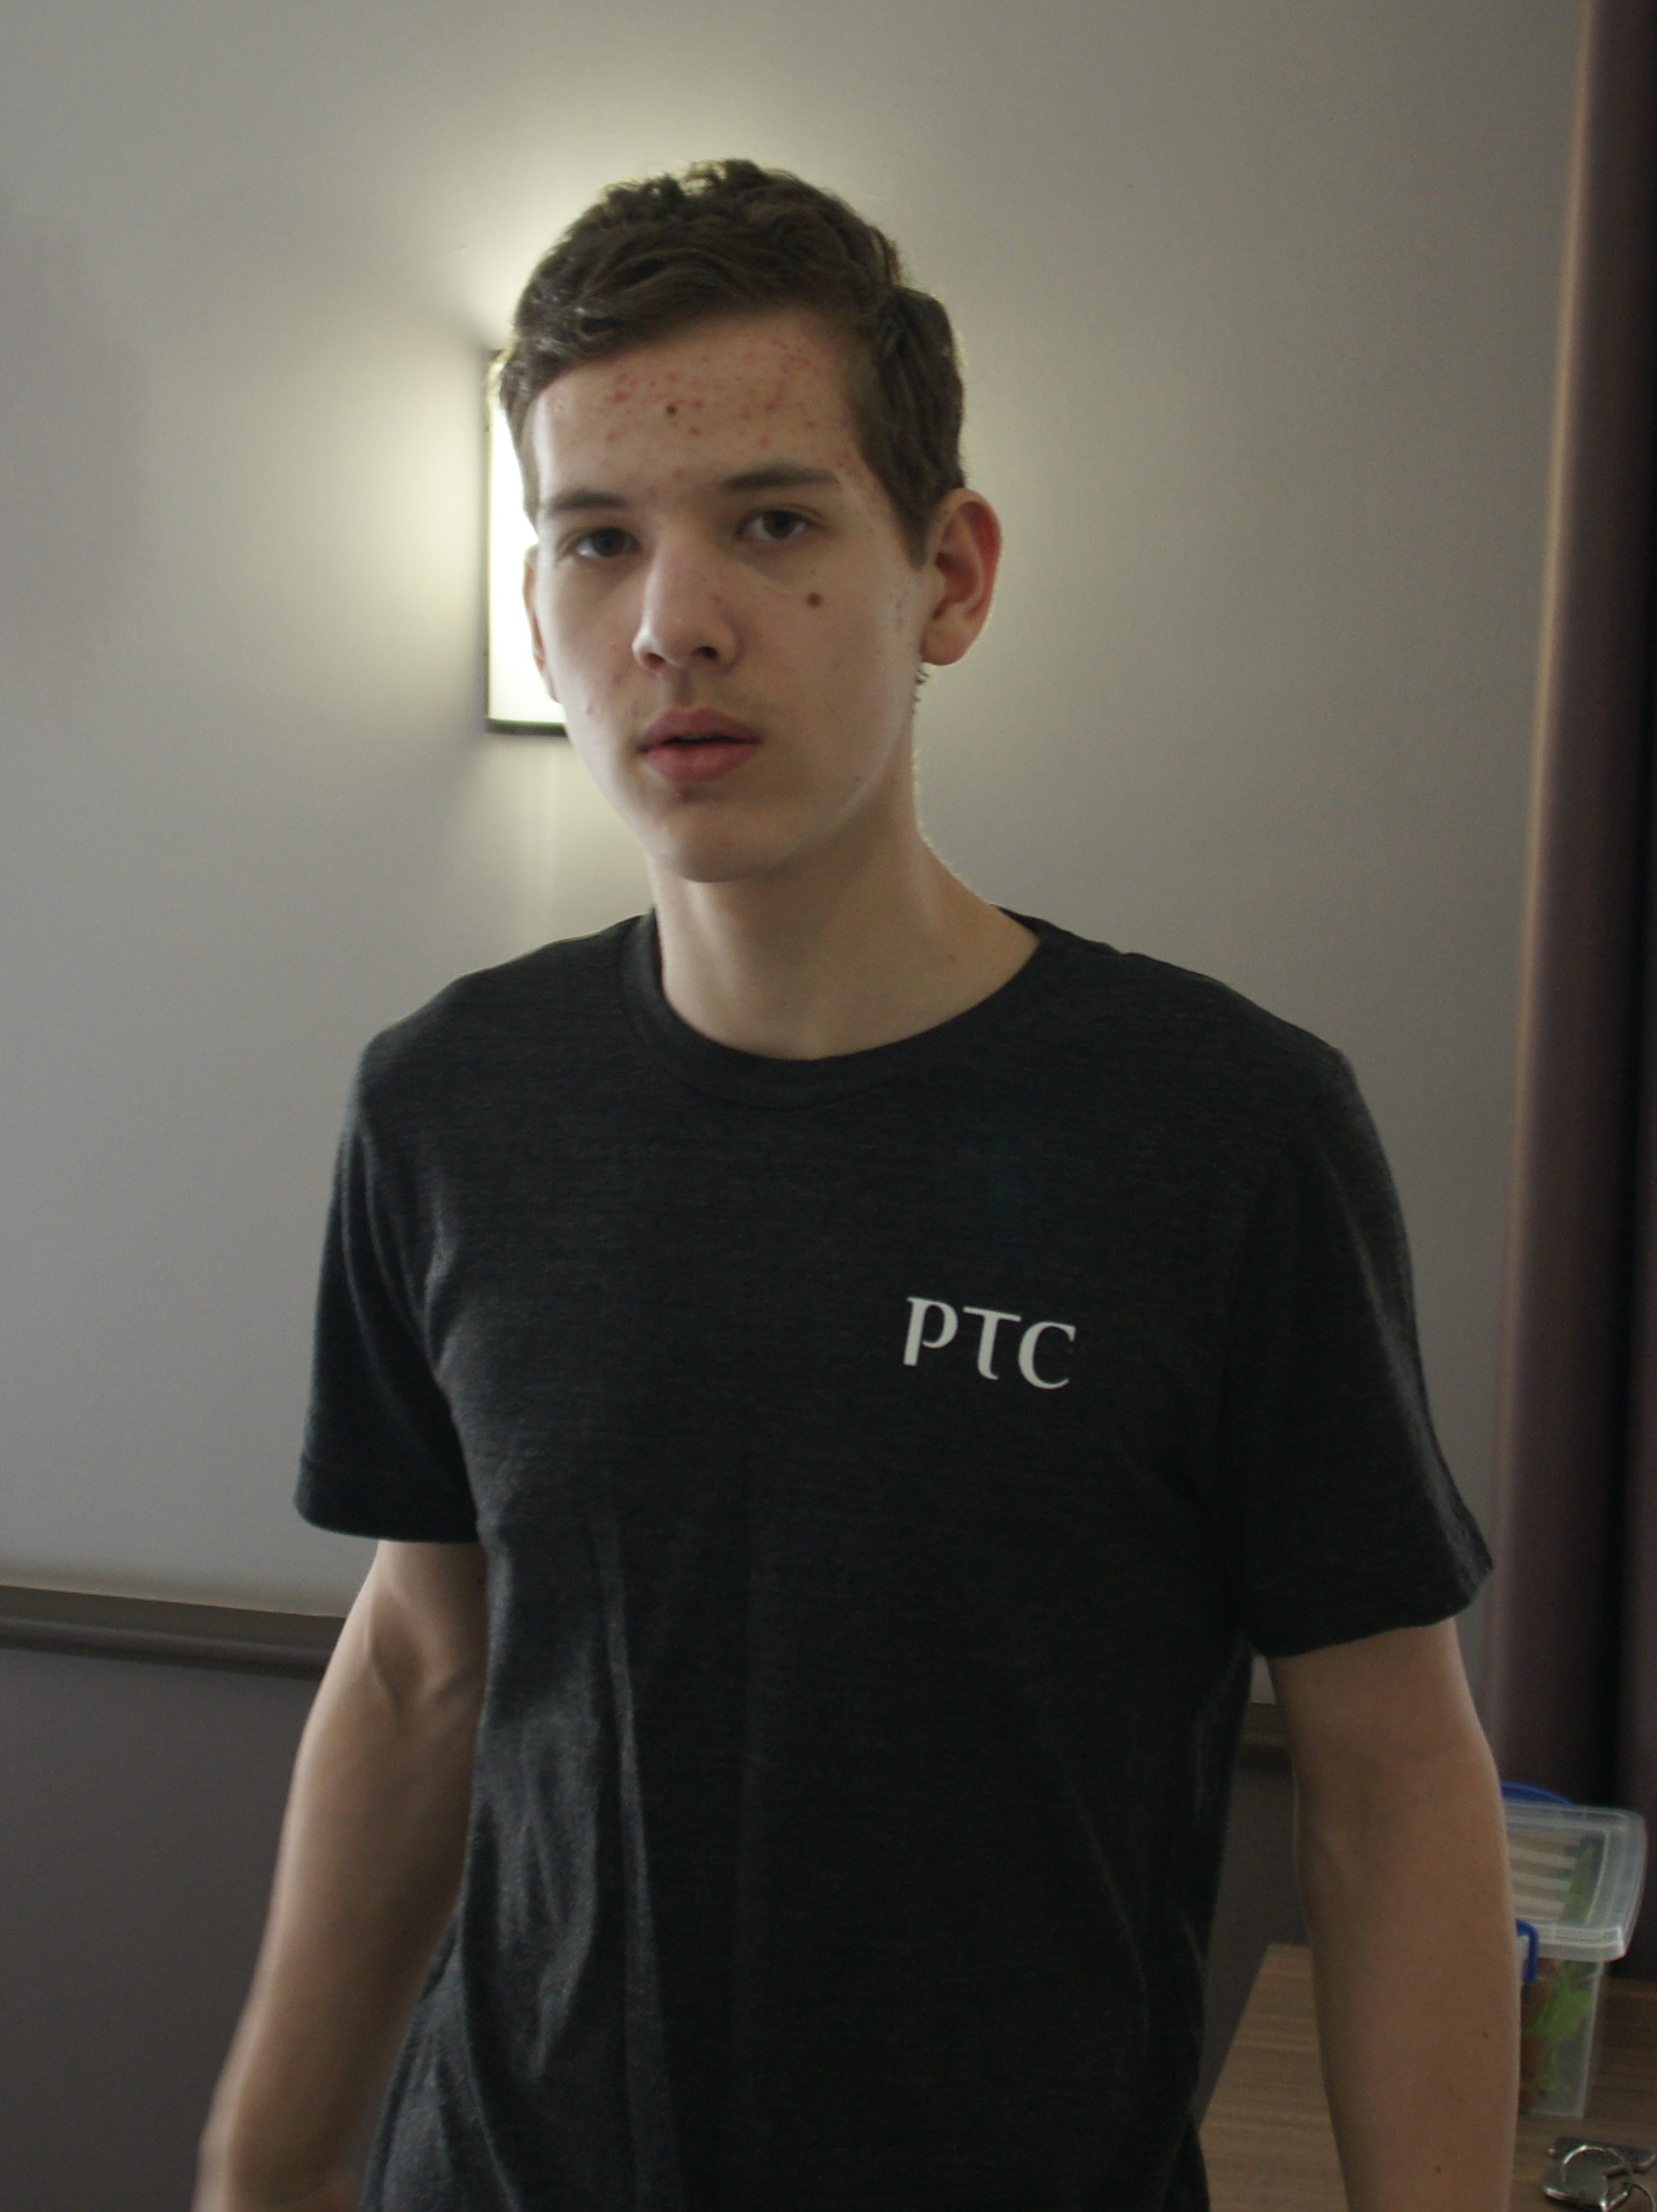
\includegraphics[scale=0.08]{days/Team/images/06}}		
	\end{minipage}
	\hfill
	\begin{minipage}[h]{0.47\linewidth}
		Krylov Georgii \\
		\emph{Part in the command: captain, coordinator of the action operators in game, responsible for the modification of robot.\\}
		\emph{Information: 17 years old, in robotics 3 years, in FTC 3 years. \\}
		\emph{Why I chose FTC: "I chose the FTC, because I like to come up with the design of robots and turn their ideas into reality, because every time I feel the Creator, who created a new creature."}		
	\end{minipage}
	\vfill 
	\begin{minipage}[h]{0.47\linewidth}
		Radionov Maxim\\
		\emph{Part in the command: communication with the team and community, decorating robot, Power Design, reserve operator. \\  }
		\emph{Information: 16 years old, in robotics 3 years, in FTC 1 year. \\}
		\emph{Why I chose FTC: "Because I like to create a robot from scratch, from somethink, I can do with my hands: cut, drill and assemble."}					
	\end{minipage}
	\hfill
	\begin{minipage}[h]{0.47\linewidth}
		\center{
\includegraphics[scale=0.25]{days/Team/images/02}}\\
	\end{minipage}
	\vfill
	\begin{minipage}{0.47\linewidth}
		\center{
\includegraphics[scale=0.22]{days/Team/images/03}}\\
	\end{minipage}
	\hfill
	\begin{minipage}{0.47\linewidth}
		Safronov Nikita\\
		\emph{Part in the command: manipulator-1,  creation of 3D models, chief engineer, responsible for the assembly robot.\\}
		\emph{Information: 16 years old, in robotics 3 years, in FTC 1 years.\\} 
		\emph{Why I chose FTC: "I have chosen FIRST because I enjoy working with mechanisms and finding unusual technical decisions for solving problems. Also working on this project helps me to get new skills in a sphere of engineering. In this case I know, that I don,t spend my time in vain."}				
	\end{minipage}
\end{figure}

\begin{figure}[H]
	\begin{minipage}{0.47\linewidth}
		Maksimychev Evgeny\\
		\emph{Part in the command: manipulator-2, responsible for the technic of safety, responsible for the writting of technical book. \\}
		\emph{Information: 15 years old, in robotics 2 years, in FTC 1 year. \\}
		\emph{Why I chose FTC: "This is an interesting project that allows to implement some innovative solutions. In addition to the skills of designing robots, we also obtain the skills of the technical documentation and communication with colleagues which makes this competition as close to real engineering problems."}			
	\end{minipage}
	\hfill
	\begin{minipage}{0.47\linewidth}
		\center{
\includegraphics[scale=0.25]{days/Team/images/04}}\\
	\end{minipage}
	\vfill	
	\begin{minipage}{0.47\linewidth}
		\center{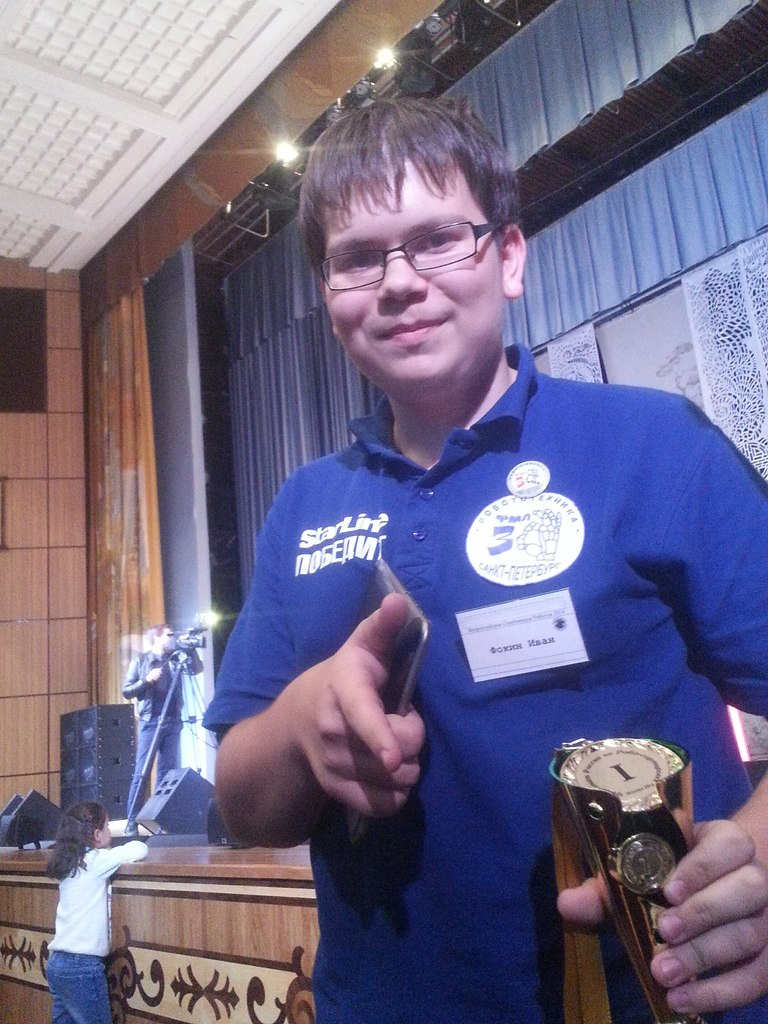
\includegraphics[scale=0.2]{days/Team/images/01}}			
	\end{minipage}
	\hfill
	\begin{minipage}{0.47\linewidth}
		Fokin Ivan\\
		\emph{Part in the command: purchase of materials,  development strategy in the game,  communication with the press, reserve  manipulator.\\ }
		\emph{Information: 17 years old, in robotics 5 years, in FTC 3 years. \\ } 
		\emph{Why I chose FTC:" When I first I attended the event FTC saw hefty metal robots, with enthusiasm and without hesitation decided that I would like to do this."}		
	\end{minipage}	
\end{figure}

\fillpage


